\documentclass[11pt]{article}
\usepackage[margin=1in]{geometry}
\usepackage{amsmath,amssymb}
\usepackage{graphicx}
\usepackage{booktabs}
\usepackage{xcolor}
\usepackage[colorlinks=true,linkcolor=blue!60!black,citecolor=blue!60!black,urlcolor=blue!60!black]{hyperref}

\title{NIRNAY: A 450M Calibrated Decision Model with Stable Product-Quantized Concepts}
\author{Eulogik\\ \texttt{info@eulogik.com}}
\date{September 30, 2026}

\begin{document}
\maketitle

\begin{abstract}
Small decision models turn a state plus a typed question into calibrated
probabilities in one forward pass. They are cheap to serve but hard to
train: we document two distinct training-collapse mechanisms in a
product-quantized concept bottleneck, both ending in constant predictions
(1/77 accuracy on Banking77). First, the encoder output grows unboundedly
(RMS 0.089 healthy, 13.5 dead) while codebook centroids stay near zero, so
the vector-quantization loss explodes $300\times$. A directional test shows
descending the task loss raises the scale while descending the
quantization loss lowers it. Second, code usage collapses to one code per
chunk (dominant share 0.97) with no loss spike at all, and the commitment
term then homogenizes encoder features. The fixes are small and structural:
an affine-free LayerNorm on the quantized input, which removes scale as a
degree of freedom, and a load-balancing auxiliary loss over hard
assignment fractions times soft assignments, whose gradients cannot
saturate at collapse. A failed entropy-based alternative is reported. A
heldout-probe safety net (periodic eval, best-checkpoint retention,
collapse abort) caught four real collapses during development. The
resulting 450M model scores \textbf{0.8792} on Banking77 test (3,080
cases, Brier 0.208, fitted ECE 0.045), against 0.803 for the Jev 1.13.0 API
on the same cases and 0.64 for the 144M Julia-1 on its easier 72-label
pilot. Code, weights, and raw eval JSONs are public under Apache-2.0.
\end{abstract}

\noindent\textbf{Keywords:} decision models, calibration, vector quantization,
concept bottleneck, load balancing, Banking77, small language models.

\section{Introduction}

Production systems need answers, not chat: which team owns this incident,
is this charge a duplicate, how urgent is this request. Decision models
take a state plus a typed question (choice, score, yes/no) and return
probabilities in one pass. The category has a clear leaderboard
(JevBench~\cite{jevbench}) and fast-moving open entries (Laya, Julia-1,
CLM-8B), but small open models keep failing in the same places: many
options, honest calibration, and stable training.

This paper reports what broke when we trained one, and the fixes that
held through a full 7,000-step run. Our contributions:

\begin{itemize}
\item Two collapse mechanisms with opposite signatures, isolated by
feature-path probes: unbounded encoder-output scale (loss spike $300\times$)
and code-usage collapse (no spike, constant predictions either way).
\item A directional-gradient test showing the task loss climbs scale while
the quantization loss pulls it down, which explains the runaway.
\item Two structural fixes: affine-free LayerNorm before quantization, and
a saturation-proof load-balancing term. Plus a documented failed attempt
(entropy deficit) with the reason it fails.
\item A probe safety net that bounds collapse damage to minutes and keeps
the best checkpoint automatically.
\item A 450M Apache-2.0 model at 0.8792 Banking77 test accuracy with fitted
ECE 0.045, with every number reproducible from shipped artifacts.
\end{itemize}

\section{Background}

Vector quantization maps continuous states to a finite codebook~\cite{vqvq}.
Concept bottleneck models route predictions through human-readable
concepts~\cite{koh2020}. Load-balancing losses of the form $K\sum fP$
keep mixture assignments spread~\cite{switch2101}. Scalar quantization
(FSQ~\cite{fsq2309}) avoids codebooks entirely; variational bottlenecks
constrain representations explicitly. For small models, process-level
supervision beats outcome-only rewards~\cite{rlvr2607}, and outcome-only
rewards fail on long-context grounding~\cite{longrlvr2603}. Activation
distributions decide quantizer behavior~\cite{infoquant2605}, and VQ
collapse is a property of the spanned space rather than single
vectors~\cite{collapse2411}. Discrete concepts can also be read off frozen
states post hoc~\cite{vqlc2602}.

We train with AdamW~\cite{adamw1711}. Calibration is reported as raw and
fitted expected calibration error on every eval, never one alone. Our
reinforcement step follows the calibrated-decision recipe (RLCD)~\cite{typesafe}. The eval
landscape: JevBench v1.5.4 ranks 106 systems over 1,624 decisions (904
open, 720 sealed) on intelligence, calibration, speed, and cost; on
2026-09-30 the board reads Cygnet 73.7, Winnow-12B 73.2 (intelligence
74.4, sealed 76.4), Jev 1.13.0 72.1 (intelligence 72.0, calibration 88.0).
Banking77~\cite{banking77} is 77-way intent classification (3,080 test
cases). Our base is Laya, a 421M Apache-2.0 decision encoder.

\section{Model}

A frozen ModernBERT-style encoder~\cite{modernbert2412} (LoRA adapters
trainable) maps token and byte inputs to hidden states $h$. A concept
bottleneck encodes $z = \mathrm{encode}(h)$ (128 dims), quantizes four
32-dim chunks against four 32-code codebooks, mixes M=4 slots, and adds a
zero-initialized residual $\delta$ back to $h$. A 2-layer head scores dense
markers; a coarse-to-fine pointer re-ranks the top 20 for 77-way rows.
Per-bucket temperatures calibrate the output. Deep supervision at layers
4/8/12 and the RLCD phase exist only in training.

The plan loss is fixed:
\begin{equation}
L = L_{\mathrm{choiceCE}} + L_{\mathrm{RPS}} + L_{\mathrm{BCE}} + L_{\mathrm{rel}}
+ 0.3\,L_{\mathrm{NCP}} + 0.2\,L_{\mathrm{deep}} + \lambda L_{\mathrm{calCE}},
\quad \lambda = 0.005,
\end{equation}
with $L_{\mathrm{NCP}} = \mathrm{codebook} + \mathrm{commitment} +
\mathrm{gateUsage}$. The optimizer has three groups: lr $5\times10^{-4}$
(rest), $10^{-5}$ (pretrained head/scorer/embeddings, 26.2M params), and
$10^{-4}$ (concepts, 4.7M). Global gradient clip 1.0. Mix: 8,412 train /
2,103 heldout (Banking77 train split plus 512 synthetic), batch 4, LoRA
rank 8, seed 13, one M4 Mac.

\section{Collapse diagnosis}

Two supervised runs died at exactly 1/77 test accuracy with different
loss signatures. A feature-path decomposition (stratified n=308) exonerated
head, scorer, and delta (each scores $\approx$0.53 on healthy encoder
features) and convicted the encoder adapters (feature std 0.44 healthy,
0.18 dead; zeroing LoRA restores features).

\textbf{Mechanism A: scale runaway.} Table~\ref{tab:scale} tracks the
encoder-output RMS on fixed probe inputs. Centroid RMS stays near 0.04
throughout, so $\mathrm{mse}(z, z_q)$ tracks $z$ and the NCP term explodes
(22.3 at step 150 in one run, 323.9 at step 75 in another, 31.5 at step
6416 in the 7,000-step run). Hidden-state RMS stays near 1.13 and encoder
weight RMS stays at init, so the growth is a gain/regime shift inside the
projection (GELU mean 0.035 to 0.529), not input or weight blowup. A
directional test at a pre-death checkpoint settles the cause: a unit step
along the task gradient \emph{raises} $z$ std (+455 per unit), while a unit
step along the NCP gradient \emph{lowers} it ($-2980$). Scale is
task-driven; the codebook chases it at full learning rate; the loop has no
fixed point. Figure~\ref{fig:collapse}(a) shows the progression.

\begin{table}[h]
\centering
\caption{Encoder-output RMS on fixed probe inputs. Centroids stay near 0.04; hidden RMS stays near 1.13.}
\label{tab:scale}
\begin{tabular}{lcccc}
\toprule
Checkpoint & $z$ RMS & centroid RMS & hidden RMS & NCP \\
\midrule
Healthy (250 steps) & 0.089 & 0.042 & 1.141 & 0.03 \\
Pre-death (25 steps) & 0.958 & 0.039 & 1.133 & 1.70 \\
Dead (50 steps) & 5.085 & 0.036 & 1.148 & 41.98 \\
Dead (75 steps) & 13.494 & 0.043 & 1.130 & 323.89 \\
\bottomrule
\end{tabular}
\end{table}

\textbf{Mechanism B: usage collapse.} With no pressure on code usage, the
per-chunk dominant share climbs (healthy 0.27 to 0.49 across 32/32 codes;
dead 0.92 to 0.99 on 2 to 14 codes). The quantized states go near-constant
and commitment homogenizes encoder directions. Crucially, a run with the
scale fix but no usage term still dies at step 75 with NCP flat near 1.9:
usage collapse alone is sufficient, and it gives no loss warning.
Figure~\ref{fig:collapse}(b) shows the progression.

\begin{figure}[h]
\centering
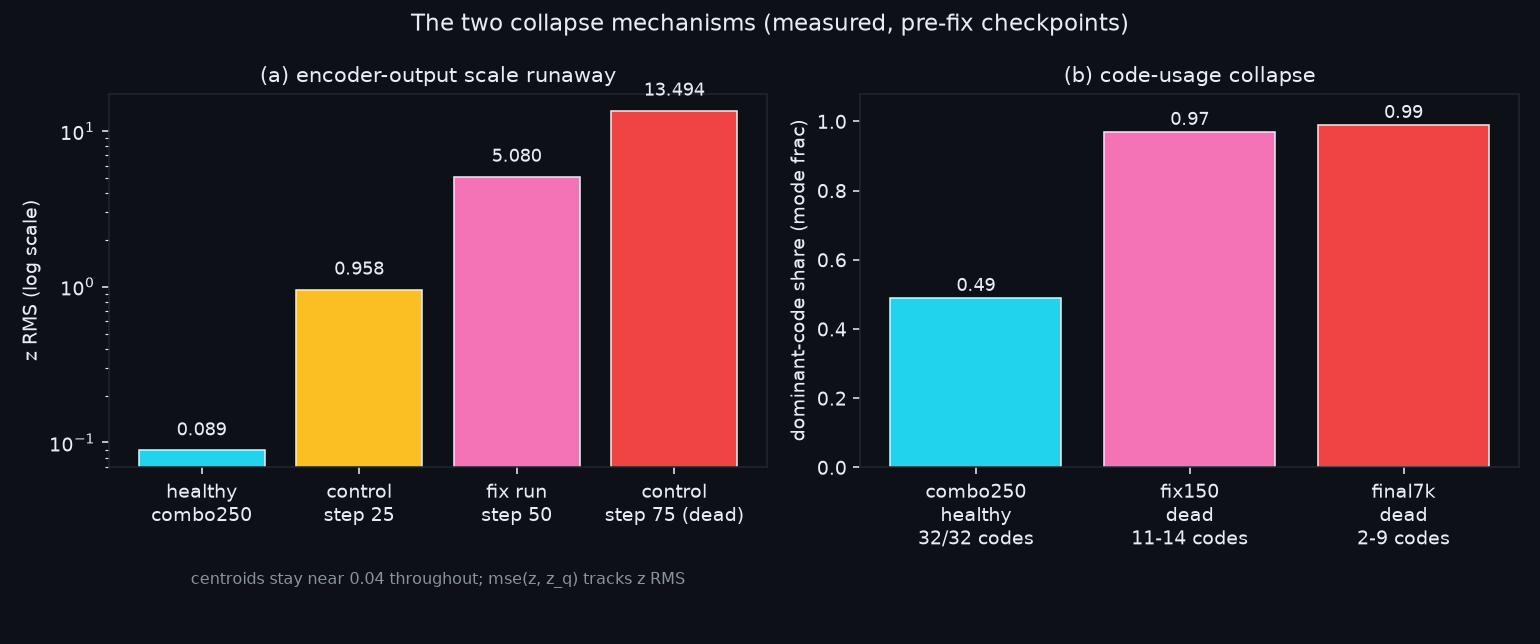
\includegraphics[width=\textwidth]{figs/collapse_signatures.png}
\caption{Measured pre-fix signatures. (a) Encoder-output scale runaway on a
log axis. (b) Code-usage collapse as dominant-code share.}
\label{fig:collapse}
\end{figure}

\section{Fixes}

\textbf{LayerNorm on $z$ before quantize} (affine-free, zero params, zero
state-dict keys, so old checkpoints still load). Scale leaves the system:
the task gradient can only rotate $z$, NCP stays $O(1)$, and assignments
become direction-based. This directly removes mechanism A.

\textbf{Load-balancing aux term.} Let $f$ be hard assignment fractions
(detached) and $P$ the mean soft assignment at temperature $\tau = 0.1$:
\begin{equation}
L_{\mathrm{usage}} = w \sum_{\mathrm{chunks}} \max(K\, f \cdot P - 1,\, 0),
\quad w = 0.01.
\end{equation}
It is linear in $P$, so gradients flow even at collapse. The first attempt,
an entropy deficit $w(\ln K - H)$, failed A/B testing twice: at $\tau=0.5$
it is too soft to see early skew (gaps near 0.08), and at sharp $\tau$ it
saturates to one-hot exactly when pressure is needed most. The failed form
is reported so nobody repeats it.

\textbf{Safety net.} Training splits into segments with a heldout probe
after each (same argmax rule as final eval), recording accuracy plus
per-chunk unique/mode statistics. Best checkpoint is retained; training
aborts when probe accuracy halves or NCP spikes. This caught four real
collapses during development and bounds any future death to minutes.

\section{Experiments}

\textbf{A/B ladder} on the known-kill config (concepts-lr $5\times10^{-4}$),
same seed throughout (Table~\ref{tab:ab}). The full fix is the only
variant that both keeps usage healthy and learns; the shipped config
(concepts-lr $10^{-4}$) then reproduces the pre-fix baseline exactly
(test 0.5218 vs 0.5195).

\begin{table}[h]
\centering
\caption{Fast-repro A/B, kill config unless noted. Acc = heldout probe.}
\label{tab:ab}
\begin{tabular}{lccc}
\toprule
Variant & Outcome & Best acc & Usage at end \\
\midrule
No fix (control) & dead at 75 (NCP 323) & 0.25 & collapsed \\
LN only, no aux & dead at 75, NCP flat & 0.22 & collapsed \\
LN + entropy aux & dead at 50 & 0.32 & collapsed \\
LN + balance aux & abort at 100, peak 0.40 & 0.40 & healthy \\
LN + balance aux, shipped lr & 250/250 clean & 0.51 & healthy \\
\bottomrule
\end{tabular}
\end{table}

\textbf{Full run.} 7,000 steps with probes: accuracy 0.28 to 0.89 (best
0.8906 at step 5000, final 0.8789), NCP flat between 1.91 and 2.01 for all
7,000 steps, usage oscillating in a stable band with the aux term pushing
back every narrowing (Figure~\ref{fig:train}). The run passed straight
through the step-6400 zone that killed its predecessor. Loss 3.93 to 1.25.

\begin{figure}[h]
\centering
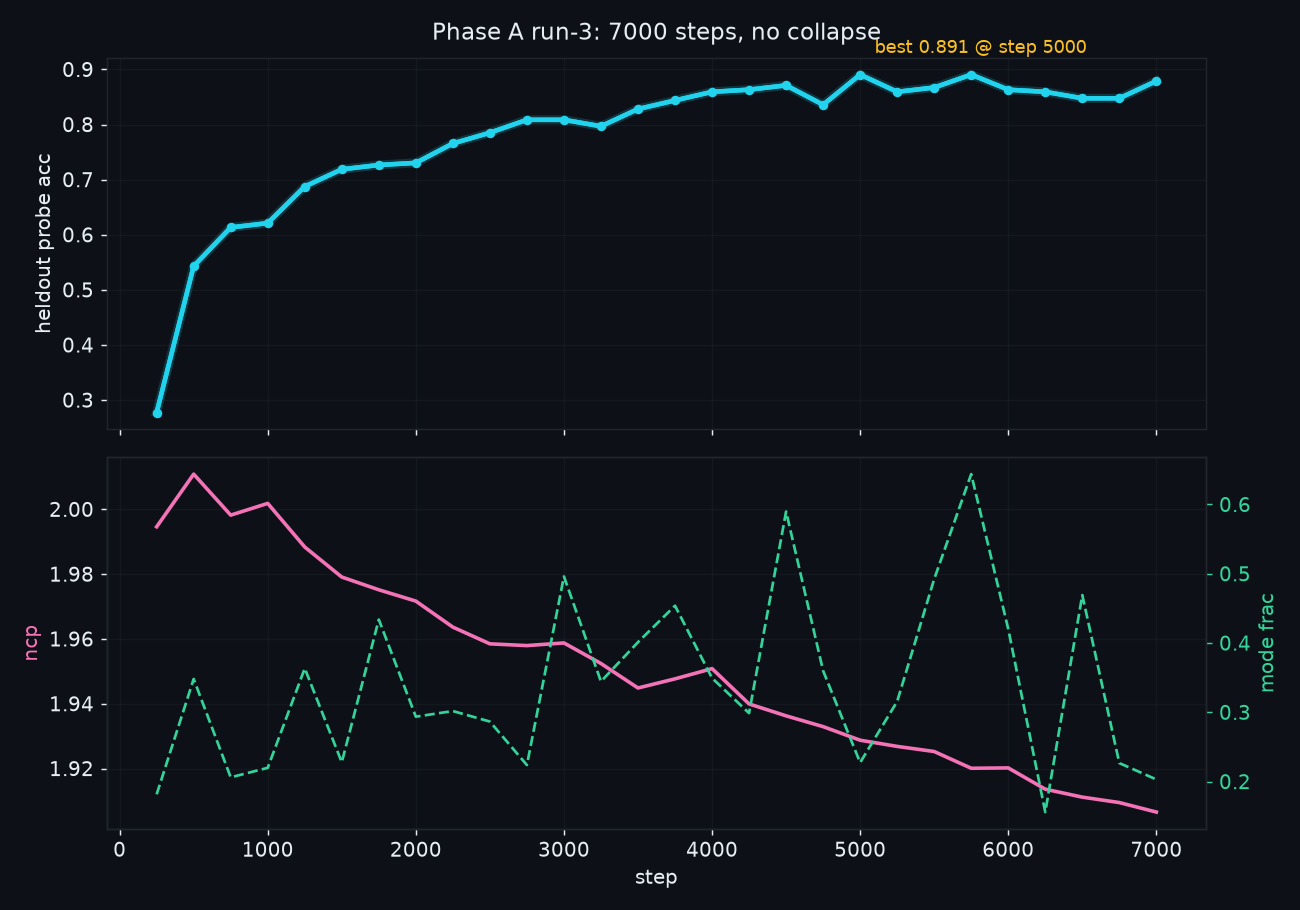
\includegraphics[width=\textwidth]{figs/training_stability.png}
\caption{Protected 7,000-step run: climbing probe accuracy, flat NCP, usage
in a self-limiting band. No storm at the historical death zone.}
\label{fig:train}
\end{figure}

\textbf{Banking77 test} (3,080 cases, Table~\ref{tab:bank} and
Figure~\ref{fig:bench}). Phase A: 0.8656 accuracy, Brier 0.240, raw ECE
0.110, fitted 0.033. Plus 50 RLCD steps (Phase B): \textbf{0.8792},
Brier 0.208, raw ECE 0.089, fitted 0.045. The best-probe checkpoint scores
lower on test (0.8542) than the final one (0.8656): probes detect collapse,
they do not fine-rank. The Jev reference ran the same 3,080 cases~\cite{jevbenchxyz}.

\begin{table}[h]
\centering
\caption{Banking77 test (n=3080). Setups stated exactly.}
\label{tab:bank}
\begin{tabular}{lccc}
\toprule
Model & Accuracy & Setup \\
\midrule
NIRNAY phase\_b & \textbf{0.8792} & fine-tuned 450M, this work \\
NIRNAY phase\_a & 0.8656 & fine-tuned 450M, this work \\
Jev 1.13.0 & 0.803 & zero-shot API, same 3,080 cases \\
Julia-1 144M & 0.64 & their 72-label pilot (n=100, shortlist) \\
Untrained & 0.1429 & fresh weights, our template \\
\bottomrule
\end{tabular}
\end{table}

\begin{figure}[h]
\centering
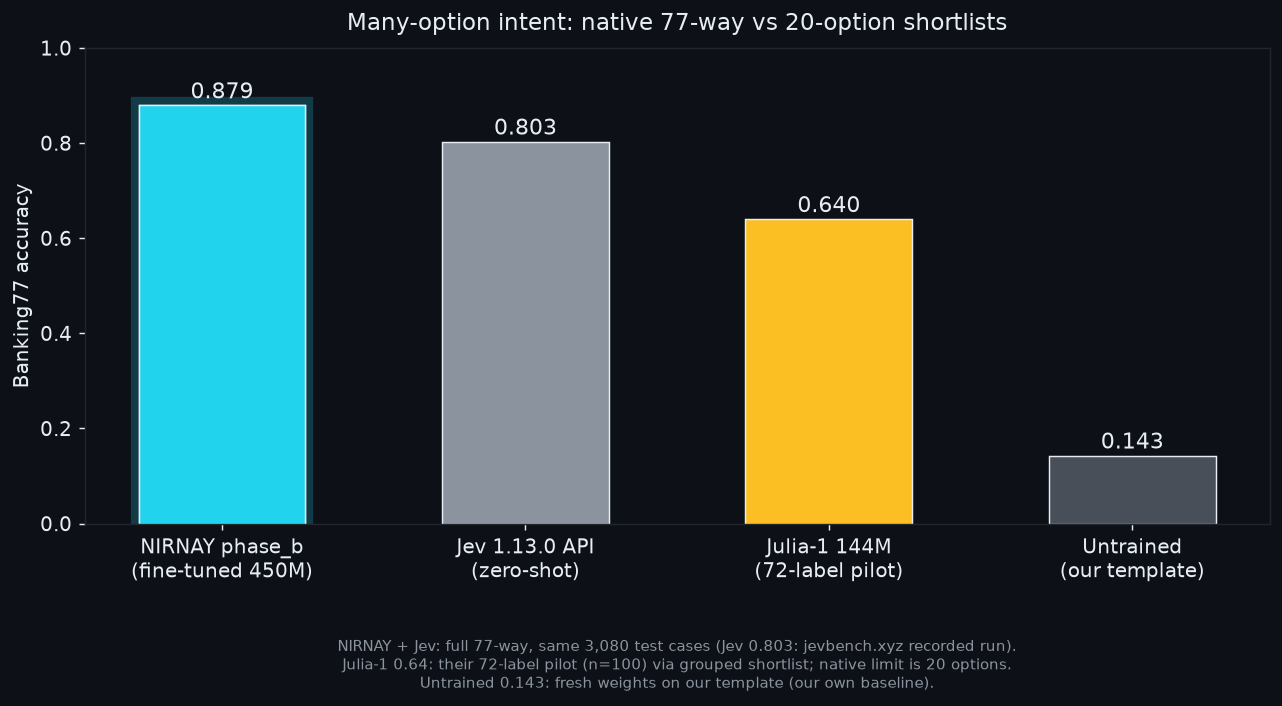
\includegraphics[width=\textwidth]{figs/benchmark_banking77.png}
\caption{Many-option intent: native 77-way against shortlists. Footnotes in
figure state every setup difference.}
\label{fig:bench}
\end{figure}

\textbf{Calibration} (Figure~\ref{fig:rel}). Most mass sits above 0.9
confidence at 92\% accuracy there; fitted ECE 0.045. Raw and fitted are
always reported together.

\begin{figure}[h]
\centering
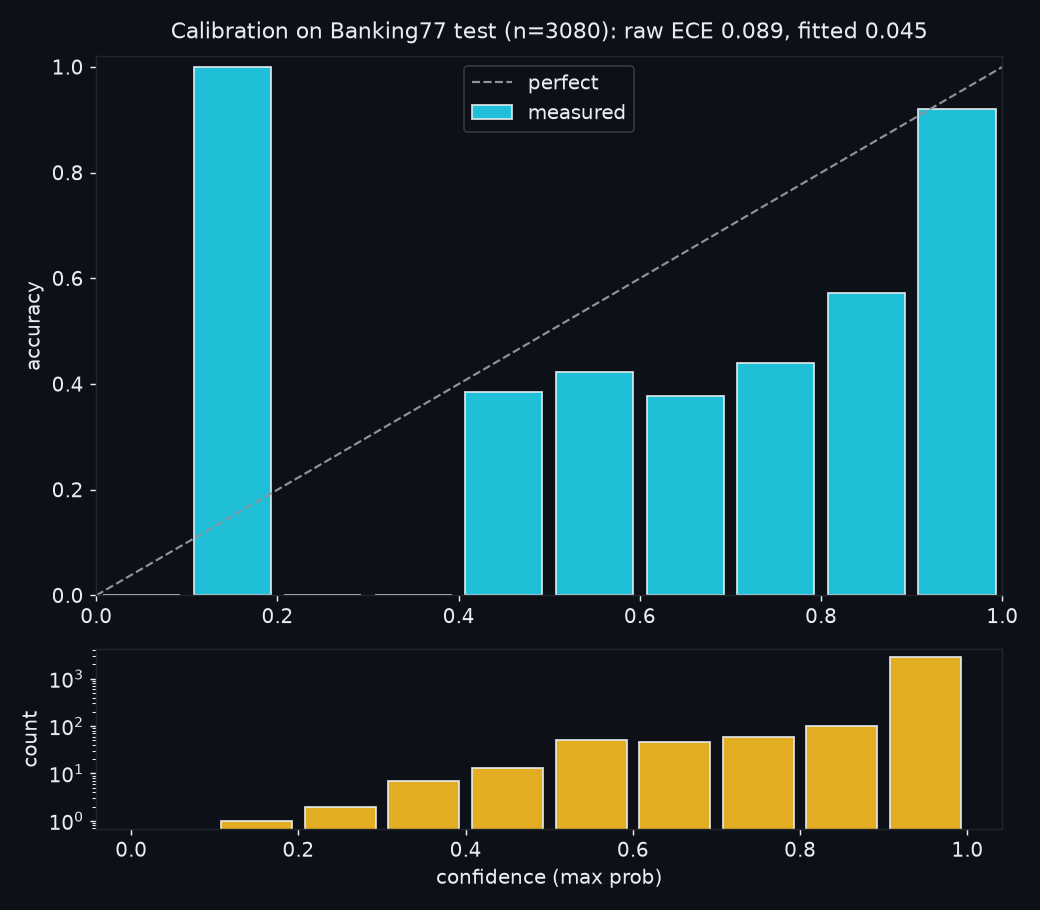
\includegraphics[width=\textwidth]{figs/reliability.png}
\caption{Reliability on Banking77 test (n=3080), measured forward pass.
Raw ECE 0.089, fitted 0.045.}
\label{fig:rel}
\end{figure}

\textbf{Honest misses.} JevBench public (231 items, shipped checkpoint):
0.550 overall (easy 0.875, original 0.569, hard 0.396). Hard states average
1,037 tokens and 63\% exceed the 320-token state budget; fitting items
still score only 0.488, so context and reasoning both gap. A head-plus-tail
windowing fix scored 0.300 against 0.343 head-only and was rejected. A
10k-item programmatic reasoning set (ground truth by construction, nothing
copied from JevBench) is built and validated but untrained at scale.

\begin{figure}[h]
\centering
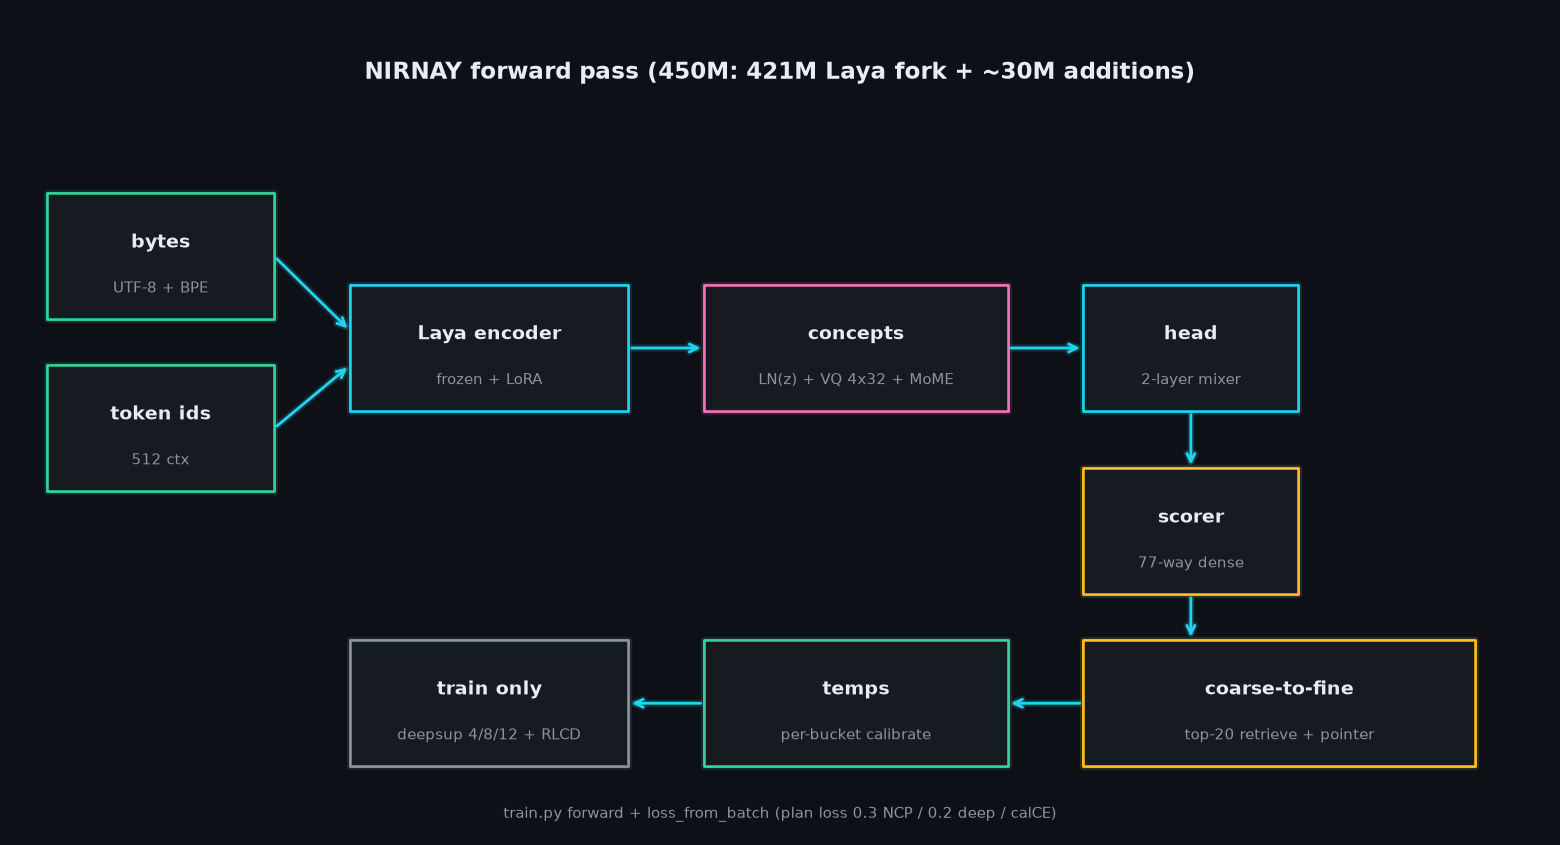
\includegraphics[width=\textwidth]{figs/architecture.png}
\caption{Forward pass: byte path, frozen encoder plus LoRA, concept
bottleneck, dense scorer, coarse-to-fine pointer, per-bucket temperatures.
Deep supervision and RLCD exist only in training.}
\label{fig:arch}
\end{figure}

\section{Related work}

VQ for concepts appears as post-hoc discovery on frozen states~\cite{vqlc2602}
(with LayerNorm around the quantizer, matching our fix), as scalar levels
without codebooks~\cite{fsq2309}, and as variational bottlenecks over
human concepts~\cite{koh2020}. Collapse is analyzed as a property of the
spanned space~\cite{collapse2411}; activation shaping is studied as
distribution design~\cite{infoquant2605}. For small-model RL, process
rewards beat outcome-only rewards at 494M parameters~\cite{rlvr2607}, and
outcome-only rewards fail long-context grounding~\cite{longrlvr2603}; our
Phase B reward is outcome-only, which bounds what it can teach.
Positioning, all numbers third-party and dated 2026-09-30: JevBench v1.5.4
ranks Cygnet 73.7,
Winnow-12B 73.2, Jev 72.1 over 106 systems~\cite{jevbench}; Laya (421M,
Apache-2.0, our base~\cite{laya}) holds $\approx$4k likes
with 33ms inference and a 56.4\% independent core score; Julia-1 (144M,
Apache-2.0~\cite{julia1}) beats Jev
on typed decisions but reports 0.64 on its Banking77 pilot and caps native
calls at 20 options;
CLM-8B (Stanford/NVIDIA, Apache-2.0~\cite{clm}) plays a GPU
tool-calling lane. Our lane is many-option
CPU classification with honest calibration, where the board is thinnest.
\section{Limits}

512-token context; 361ms CPU per decision in PyTorch (no ONNX yet, no GGUF
yet); JevBench-hard reasoning as reported; best-probe checkpoints do not
necessarily test best.

\section{Reproducibility}

Code, weights (phase\_b, Apache-2.0), frozen data hashes, all gate checks
(19/19), and raw eval JSONs ship with the release. Seeds fixed (13);
hardware one M4 Mac. Nothing in this paper comes from closed APIs.
Delivered-error claims rest on external ground-truth audits only~\cite{cheap2609}.

\begin{thebibliography}{99}

\bibitem{vqvq} A.\ van den Oord, O.\ Vinyals, K.\ Kavukcuoglu.
\textit{Neural Discrete Representation Learning.} NeurIPS 30, 2017.
arXiv:1711.00937.

\bibitem{koh2020} P.\ Koh et al.
\textit{Concept Bottleneck Models.} ICML 2020, PMLR 119.

\bibitem{switch2101} W.\ Fedus, B.\ Zoph, N.\ Shazeer.
\textit{Switch Transformers.} JMLR 2022. arXiv:2101.03961.

\bibitem{adamw1711} I.\ Loshchilov, F.\ Hutter.
\textit{Decoupled Weight Decay Regularization.} ICLR 2019.
arXiv:1711.05101.

\bibitem{banking77} I.\ Casanueva et al.
\textit{Efficient Intent Detection with Dual Sentence Encoders.}
arXiv:2003.04807.

\bibitem{modernbert2412} B.\ Warner et al.
\textit{Smarter, Better, Faster, Longer: A Modern Bidirectional Encoder.}
arXiv:2412.13663.

\bibitem{vqlc2602} X.\ Yu et al.
\textit{Vector Quantized Latent Concepts.} arXiv:2602.02726.

\bibitem{collapse2411} H.\ Siuzdak et al.
\textit{Addressing Representation Collapse in Vector Quantized Models with
One Linear Layer.} arXiv:2411.02038.

\bibitem{fsq2309} F.\ Mentzer et al.
\textit{Finite Scalar Quantization: VQ-VAE Made Simple.} ICLR 2024.
arXiv:2309.15505.

\bibitem{infoquant2605} K.\ Li et al.
\textit{InfoQuant: Shaping Activation Distributions for Low-Bit LLM
Quantization.} arXiv:2605.26175.

\bibitem{rlvr2607} A.\ Palandye et al.
\textit{Reward Granularity in RLVR for Small Language Models.}
arXiv:2607.02869.

\bibitem{longrlvr2603} G.\ Chen et al.
\textit{LongRLVR.} ICLR 2026. arXiv:2603.02146.

\bibitem{cheap2609} D.\ Rajput et al.
\textit{Cheap Verifiers, Large Blind Spots.} arXiv:2609.01345.

\bibitem{jevbench} Benchmark Heaven. \textit{JevBench v1.5.4 leaderboard.}
\url{https://benchmarkheaven.com/jev-models}, 2026-09-30.

\bibitem{jevbenchxyz} JEVBench. \textit{Recorded run: jev-1.13.0 on
Banking77 (3,080 cases).} \url{https://jevbench.xyz}, 2026.

\bibitem{laya} ConvAI Innovations. \textit{Laya multilingual decision model.}
\url{https://huggingface.co/convaiinnovations/laya}, 2026.

\bibitem{julia1} Supersonic Labs. \textit{Julia-1 decision model.}
\url{https://huggingface.co/SupersonicLabs/Julia-1}, 2026.

\bibitem{clm} Stanford / NVIDIA. \textit{Contrastive-LM/CLM.}
\url{https://github.com/Contrastive-LM/CLM}, 2026.

\bibitem{typesafe} TypeSafe AI. \textit{Introducing System One Models and
Jev (RLCD).} \url{https://typesafe.ai/blog/introducing-system-one-models-and-jev},
2026.

\end{thebibliography}

\end{document}
